\documentclass[a4paper,10pt]{article}

\usepackage{fancyhdr} % clears the header and footer setting
\usepackage{graphicx} 
\usepackage{geometry}
\geometry{a4paper, left=2cm, right=2cm, top=1.5cm, bottom=3cm }
\usepackage{caption}
\usepackage{subcaption}
\usepackage{hyperref, url}
\usepackage[natbibapa]{apacite}
\usepackage{amsmath}
\usepackage{float}
\usepackage{natbib}


\usepackage{etoolbox,fancyhdr,xcolor}
\newcommand{\headrulecolor}[1]{\patchcmd{\headrule}{\hrule}{\color{#1}\hrule}{}{}}
\newcommand{\footrulecolor}[1]{\patchcmd{\footrule}{\hrule}{\color{#1}\hrule}{}{}}
\renewcommand{\headrulewidth}{1pt}
\headrulecolor{black!100}%
\renewcommand{\footrulewidth}{1pt}
\footrulecolor{red!100}%

\fancyhf{}
\fancyhead[R]{
\includegraphics[width=0.25\textwidth]{figures/nmims.png}}

\fancyfoot[C]{Nilkamal School of Mathematics, Applied Statistics & Analytics}
\fancyfoot[R]{\thepage}

\setlength{\headheight}{15mm}
\pagestyle{fancy} %This command sets the page style to fancy, applying the header and footer configurations defined above to the document pages.

\bibliographystyle{apacite}
\setcitestyle{numbers}

\usepackage{times}
\begin{document}

\noindent 
\begin{center}
\textbf{{\Large Movie Recommendation System Using Collaborative Filtering and Content-Based Filtering}} \\
\end{center}

\noindent 
\begin{center}
\textbf{ Zaamena Shamji, Neha Maheshwari, Anushka Jain, Nitya Verma, Aditee Gupta } 
\end{center}\\[-0.5cm]

\begin{center}
\textit{Narsee Monjee Institute Of Management Studies, Mumbai}\\
\end{center}


\noindent 
\begin{center}
    \subsection*{ABSTRACT}
        The growing volume of data and information overload makes it burdensome for people to filter relevant information. Recommendation system helps solve this issue of choosing and extracting preferred information. This paper focuses on the multiple recommendation systems and building one for movies. It was founded that different recommendation system algorithms produce different results for the same movie. 


\noindent 
\textbf{KEYWORDS:} \textit{Collaborative Filtering},\textit{Content-Based Filtering},\textit{Singular Value Decomposition}
\end{center}

\section{INTRODUCTION}
With the increasing growth of content on over-the-top platforms, users often face information load and get overwhelmed. This makes it difficult for the users to choose content that is relevant to their preferences and a one-size-fits-all approach may not be effective. A recommendation system aids diverse users in getting recommendations according to individual tastes and preferences. It helps users narrow down the wide and confusing horizon of options and saves them the time and effort to go through each and every product. This not only helps users get a personalized experience but also assists them in discovering new content that would have been otherwise overlooked due to popular content.


The research objective is to develop and understand the workings and usage of a movie recommendation system. A recommendation system refers to a platform or an engine that provides suggestions for items. The purpose of the recommendation system is to suggest items or products of interest to the users. It studies the relationship between the items and the users to give specific recommendations.

    Highly regarded companies like Amazon, Netflix and Spotify use these methods to enhance their customer experience. Their recommendation system utilizes the user's interaction history, their preferences and their similarity with other users to provide recommendations.
    
    For movie recommendations, the project utilizes two types of techniques to provide personalized and relevant suggestions to the users:

\begin{enumerate}
    \item Content-Based Filtering: This method utilizes the past behaviour of the user, to suggest products that are similar to the previously used product of the user. Attributes such as genre, director, actors and generated tags or keywords are analyzed to identify similarities between movies.
    
\begin{figure}[H]
\centering
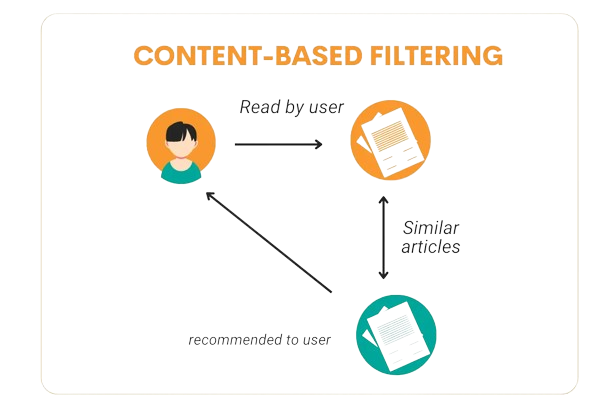
\includegraphics[height=6cm]{figures/content.png}
\caption{Content Based}
\label{content}
\end{figure}

    \item  Collaborative Filtering: As for collaboration, instead of finding similarities between the items based on the user behaviour, it finds similarities between multiple users and cross-suggests their products to each other. This technique further bisects into two approaches, namely, item-based filtering and user-based filtering.

          a)  Memory-Based Collaborative Filtering:This method helps generate recommendations by considering the ratings and preferences of similar users or the similarities between movies. It has two main approaches:
\vspace{2pt}
  
    \begin{itemize}
        \item Item-based Collaborative Filtering: This focuses on the similarities between the items or the products. Any items sharing similar features are cross-recommended to users who like either of the products.
    \end{itemize}

    \begin{itemize}
        \item User-based Collaborative Filtering: This technique recommends movies based on the similarities between users. The similarity is calculated with the help of users’ past interactions with the movies.
    \end{itemize}

    
\begin{figure}[H]
\centering
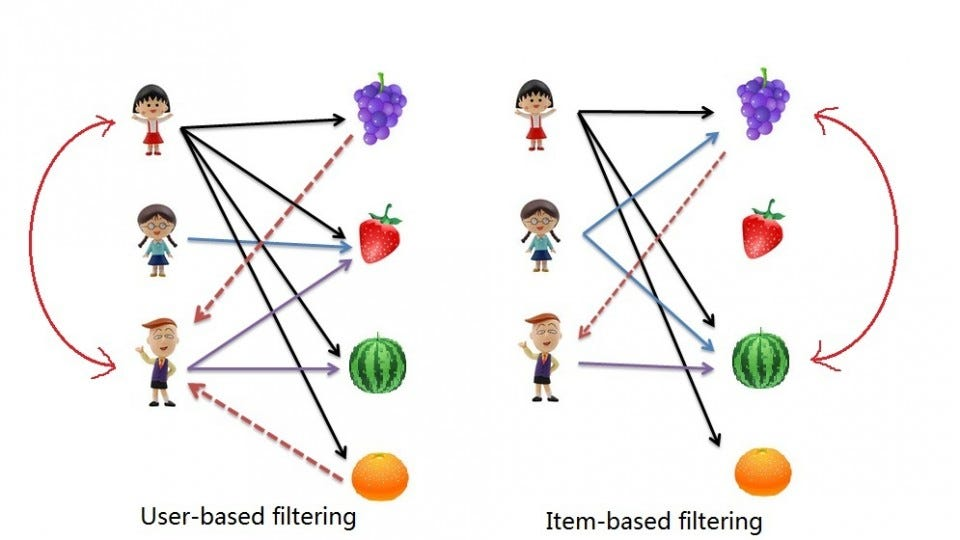
\includegraphics[height=6cm]{figures/user_item.png}
\caption{User-Based and Item-Based Collaborative Filtering }
\label{user_based}
\end{figure}

   b) Model-based Collaborative Filtering:  This method helps to predict similar movies according to users' past interactions as well as other users who are similar to them. This technique requires matrix factorization, which decomposes the user-item interactions to represent latent features.

   Similar to how numbers can be decomposed into their factors, a matrix can also be factorised into smaller matrices. Singular Value Decomposition is one such method with no restrictions on the shape and properties of a matrix that has to be decomposed. 



\begin{figure}[H]
\centering
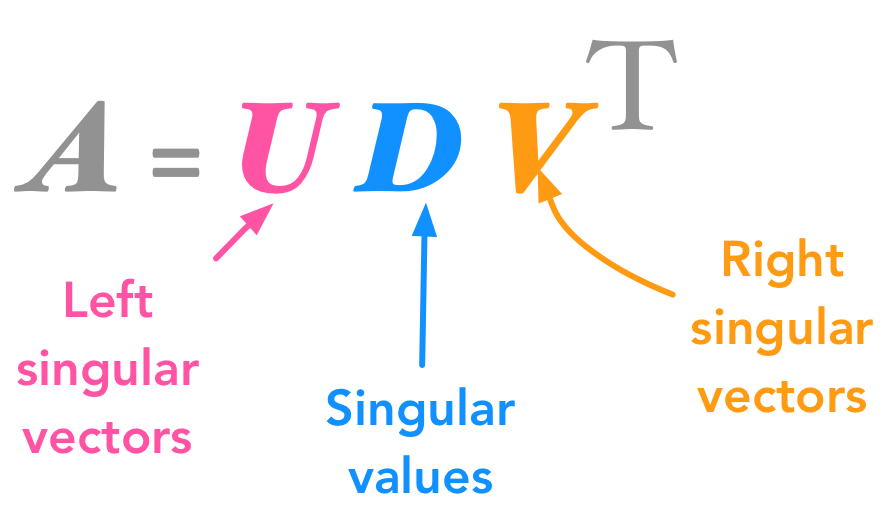
\includegraphics[height=5cm]{figures/svd.png}
\caption{Singular Value Decomposition}
\label{SVD}
\end{figure}

    The columns of matrix U are eigenvectors of \(A.A^T\) and the rows of the matrix \( V^T \) are eigenvectors of\(A^T.A\)   Now both \(A^T.A\) and \(A.A^T\) are potentially in different sizes (because the matrix can be non-square shape), but they have the same set of eigenvalues, which are the square of values on the diagonal of \(Sigma\)

    \item  Hybrid Recommendation: This method combines various techniques, such as content-based and collaborative filtering to generate more accurate and diverse recommendations. It helps to aid the limitations of individual techniques and improve the quality of recommendations.

 
\end{enumerate}
    
By employing the techniques given in figure \ref{Intro}, the research aims to improve user satisfaction and engagement. This will help the platform to increase viewership and potentially increase revenue.

\begin{figure}[H]
\centering
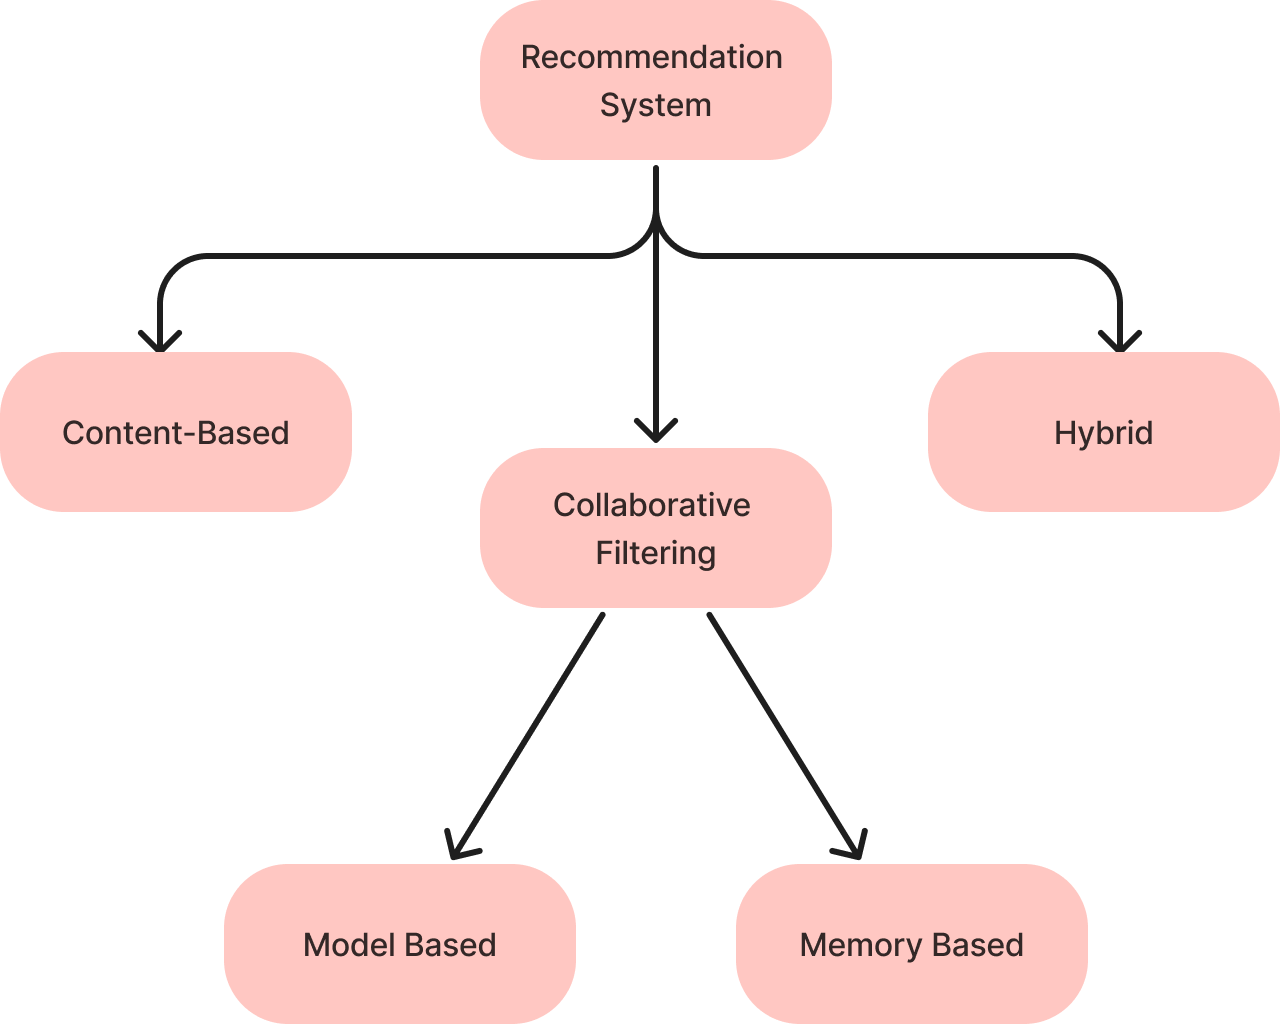
\includegraphics[height=6cm]{figures/Intro.png}
\caption{Types of Recommendation Systems}
\label{Intro}
\end{figure}



\section{LITERATURE REVIEW}

In this growing era of technology, the biggest boon is the availability of data. Information can be found everywhere with just by a few clicks of the button. Such vast and easy accessibility of data leads to perplexity \cite{Yeole2021}. Ordering this information according to the liking of the user makes it easier to skim through it. That is the exact purpose of a recommendation system. Understanding customer's behaviour and preferences makes it all the more easier for a particular website to display the appropriate data. Websites like Netflix, Amazon, and YouTube use algorithms which help in making better suggestions. 
\vspace{4pt}

Algorithms like collaborative filtering have been gaining attention from researchers and companies as it ensure the privacy of data \cite{chenna2020}. The dilemma of what to choose increases rapidly when there is a lot to choose from, and solving this particular issue is the ultimate goal of recommendation systems. This paper aims to understand various algorithms and choose the most effective one among them. \cite{chenna2020} studied the algorithm which not only recommends a movie but also reduces privacy concerns. They measured the effectiveness of the algorithms by means of various accuracy measures. 

\vspace{3pt}

\cite{roy2022} performed a systematic review to understand the various applications of recommendation systems and to deep dive into the workings of these algorithms. Various problems are present in the recommendation systems which are currently being used. Problems like the Cold start problem which occurs when a new user joins the database and the algorithm is unaware of his/her preferences. Sometimes there are very few ratings given by the active user which leads to the problem of sparsity. \cite{roy2022} found that most of the research papers focused immensely on recommendation systems for movies and only a few paid heed to other applications like tourism. This is a potential research gap found by them

\vspace{4pt}

\cite{5232419} builds a model by combining three algorithms to attain the best result. To fill the missing values in the ratings column, they employed memory based collaborative filtering whereas to make a prediction of the rating, model model-based rating was incorporated. Eventually, it was found that memory based collaborative filtering gave the most accurate results. Even though model based collaborative filtering is employed by many recommendation systems, it might limit the range of users. Although the drawbacks of memory-based collaborative filtering can be overcome by the model based collaborative filtering, but combining these models will give the best results


\vspace{4pt}

Most of the research papers revolved around the use of collaborative filtering techniques but \cite{vilakone2018} found an approach other than the same old techniques.K-cliques which are generally used in social network analysis are used in this study to build a movie recommendation system. It was found that when the value of k was kept at 11 for rating 200 movies gave the most accurate results. Five movies were recommended to the user by the means of this method


\section{DATA}

\subsection{Data Collection}

Secondary research was conducted for this project. \textbf{Netflix Prize Dataset} and \textbf{Netflix Titles} datasets were taken into account for building the recommendation system. Both datasets are available on Kaggle \cite{kaggle}. The "Netflix Prize" dataset is the official dataset published by Netflix for an open competition. The purpose of the competition was to find the best algorithm which predict the ratings of the customers. The dataset provided by the company contained only minimal information. 

The "Netflix Titles" dataset is an entirely different dataset containing detailed information about each movie.

\subsection{Data Structure}

\textbf{\textit{Netflix Prize Data}} comprises of two text file. The first dataset contains information of the ratings given by the customer to each movie. Table \ref{Data_1} shows the structure of the dataset wherein 

\begin{itemize}
  \item MovieIDs: The unique ID assigned to each movie. It ranges from 1 to 17023 sequentially.
  \item CustomerIDs: The unique ID assigned to each customer. It range from 1 to 2649429, with gaps.
  \item Ratings: Ratings given by each customer. They are on a five-star (integral) scale from 1 to 5.
  \item Dates have the format YYYY-MM-DD.
\end{itemize}
The table shows the ratings given by three different customers to movie Id 1 on the given dates. 



\begin{table}[H]
    \center 
    
    \begin{tabular}{|c|c|c|c|} \hline 
         Customer ID&  Movie ID&  Rating& Date\\ \hline 
         1488844&  1&  3& 2005-09-06
\\ \hline 
         822109&  1&  5& 2005-05-13
\\ \hline 
         885013&  1&  4& 2005-10-19
\\ \hline
    \end{tabular}
    \caption{Customer Rating}   
    \label{Data_1} 
\end{table}

The second dataset contains the titles of the movies corresponding to their respective movie IDs. Table \ref{Movie_titles} shows the structure of the \textit{\textbf{movie titles}} dataset. 

\begin{table}[H]
    \centering
    \begin{tabular}{|c|c|l|} \hline 
         Movie ID& Year Of Release&Title\\ \hline 
         1& 2004&Dinosaur Planet\\ \hline 
         48&  2001&Justice League\\ \hline 
         198
&  1997&Gupt\\ \hline
    \end{tabular}
    \caption{Movie Titles Dataset}
    \label{Movie_titles}
\end{table}

\vspace{10pt}
Figure \ref{netflix titles} shows \textbf{\textit{Netflix Titles}} dataset which contains information of the movies/TV shows on Netflix. The dataset contains \textbf{8807} movies in total. The features in the dataset are as follows 
\begin{itemize}
    \item \textbf{Show ID}: Unique ID for every Movie / TV show. 
    \item \textbf{Type}: Identifies whether it is A Movie or TV Show 
    \item \textbf{Title} :Title of the Movie / Tv Show 
    \item \textbf{Director}: Director of the Movie
    \item \textbf{Cast}: Actors involved in the movie / show
    \item \textbf{Country}: Country where the movie/show was produced
    \item \textbf{Date} Added: Date it was added on Netflix
    \item \textbf{Release} \textbf{Year}: Actual Release year of the move / show
    \item \textbf{Rating}: TV Rating of the movie / show
    \item \textbf{Duration}: Total Duration - in minutes or number of seasons
    \item \textbf{Listed In}: Genre of the movie/ Show
    \item \textbf{Description}:The summary description 
\end{itemize}
\begin{figure}[H]
    \centering
    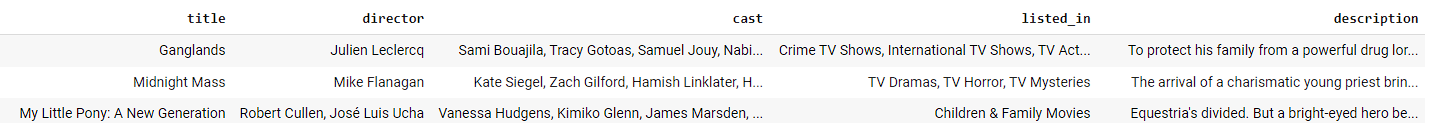
\includegraphics[width=1\linewidth]{figures/netflix_title.png}
    \caption{Netflix Titles Dataset}
    \label{netflix titles}
\end{figure}


\subsection{Exploratory Data Analysis}
The figure \ref{genre} shows the top 10 genres present in the \textit{Netflix Titles} dataset. Most of the movies are of \textbf{\textit{Drama}} category

\begin{figure}[H]
    \centering
    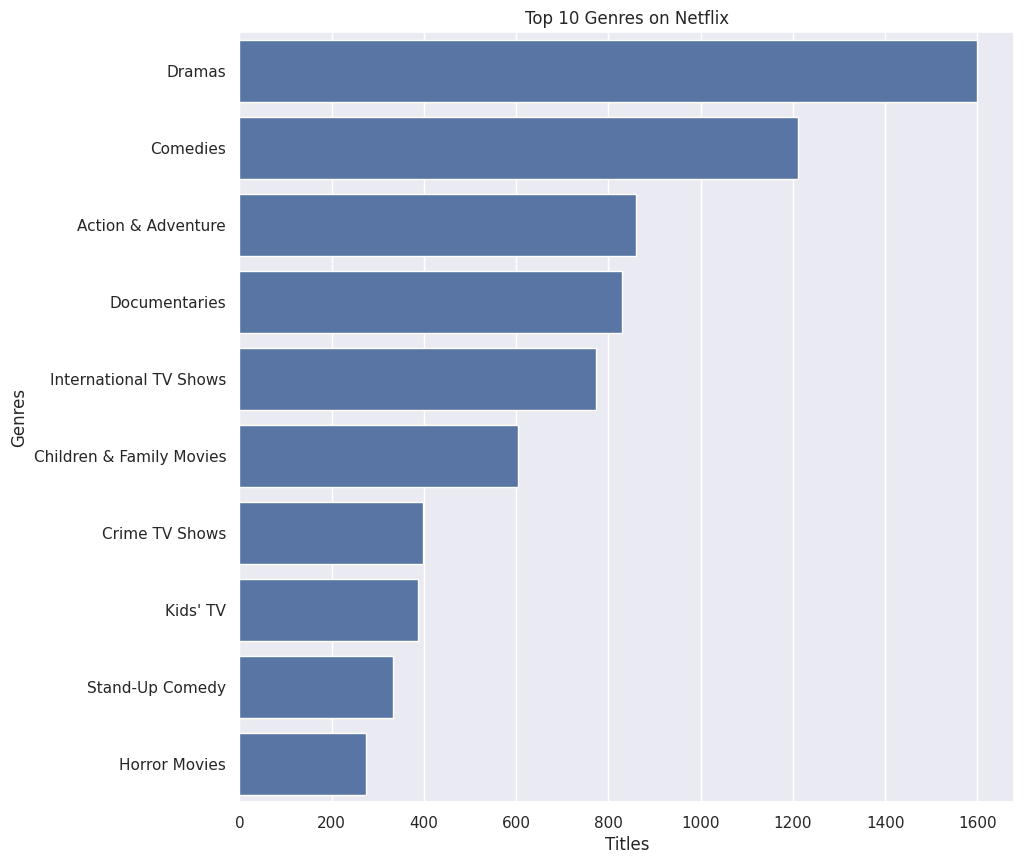
\includegraphics[width=12 cm]{genre.png}
    \caption{Top 10 Genres}
    \label{genre}
\end{figure}

\vspace{2pt}
Figure \ref{highest} shows the highest rated movie amongst the ones which have the ratings as 5. American Beauty has the highest count of 5 star ratings

\begin{figure} [H]
    \centering
    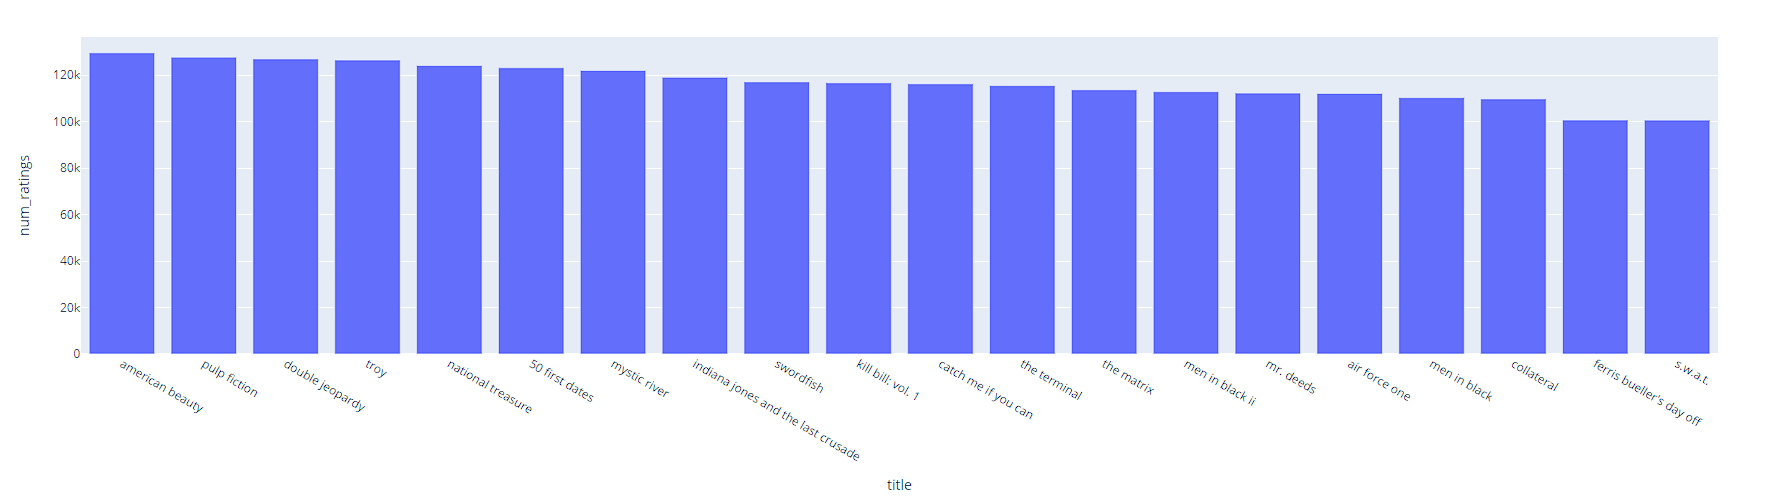
\includegraphics[width=15 cm]{highest_rated.png}
    \caption{Highest Rated Movie}
    \label{highest}
\end{figure}
\section{Methodology and Analysis}

\subsection{Data Cleaning}

All the datasets were checked for missing and duplicate values. 
The unnecessary columns like \textit{Date}, \textit{Year Of Release}, \textit{Duration}, etc were deleted. The missing values were either replaced by an empty string, in the case of attributes, or by a zero in the case of numerical columns.  
The textual data was converted into lower case in order to bring uniformity.

\subsection{Data Preprocessing}

\subsubsection{Collaborative Filtering}
\textit{\textbf{Netflix Prize dataset}} was used for item-based collaborative filtering. 
\begin{itemize}
    \item \textbf{Merging}: The two datasets (\ref{Data_1} and \ref{Movie_titles}) within the Netflix prize dataset were merged based on the common attribute \textit{MovieID}. The new dataset is given in the figure \ref{Movie_merge}
\end{itemize}

\begin{figure}[H]
\centering
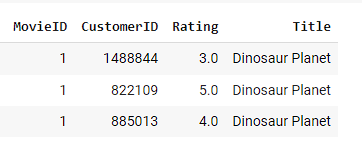
\includegraphics[height=3.5cm]{figures/movie_data.png}
\caption{Merged Data}
\label{Movie_merge}
\end{figure}


\begin{itemize}
    \item \textbf{Outliers}: The count of ratings given to each movie was calculated. The average count of ratings turned out to be around 26. The outliers were removed by the given formula 
\end{itemize}

\begin{enumerate}
  \item Interquartile Range (IQR):
    \[ \text{IQR} = Q3 - Q1 \]

  \item Upper Limit for Outliers:
    \[ \text{Upper Bound} = Q3 + 1.5 \times \text{IQR} \]
\end{enumerate}

\subsubsection{Content Based Filtering}:

\textbf{\textit{Netflix Titles}} \ref{netflix titles} was used to for content based filtering

\begin{itemize}
    \item \textbf{Stop word removal}: Stopwords are those words which do not add any meaning to the data and are used only to make sense of the information. Words like \textit{a}, \textit{an}, \textit{the}, etc are considered as stopwords. Such words can be removed from the data to increase computational efficiency. 
\end{itemize}


\begin{itemize}
    \item \textbf{Vectorization}: For algorithms to understand textual data, vectorization is used to convert any such data into a numerical value. Vectorization is a natural language processing technique. There are many different methods to perform this process like Bag of Words, TF-IDF, and Word2Vec.We have used Bag of Words to vectorized our data
\end{itemize}

\begin{itemize}
    \item \textbf{Stop word removal}: Stopwords are those words which do not add any meaning to the data and are used only to make sense of the information. Words like \textit{a}, \textit{an}, \textit{the}, etc are considered as stopwords. Such words can be removed from the data so as to increase computational efficiency
\end{itemize}

\begin{itemize}
    \item \textbf{Stemming}: Stemming refers to the process of conversion of words to their base/root form. For example, learn, learning, learned etc have the same meaning, hence they can be converted into their root form that is \textit{learn}. Stemming also helps increase the accuracy and reduces duplication. 
\end{itemize}



\subsection{Collaborative Filtering}

\begin{enumerate}
    \item \textbf{Item-based}: 
    \vspace{2pt}
    \begin{itemize}
        \item  \textbf{\textit{STEP 1: User Matrix}}
        \vspace{2pt}
        This step focuses on building the user-movie correlation matrix based on the ratings given by users to all the movies. Figure \ref{user_movie} shows the user-movie matrix 

\begin{figure}[H]
    
        \centering
        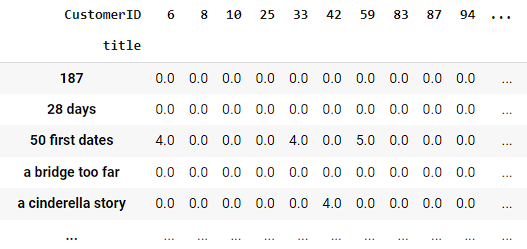
\includegraphics[height=3.5cm]{figures/user_movie.png}
        \caption{User Movie Matrix}
        \label{user_movie}
        
\end{figure}
 
    \item  \textbf{\textit{STEP 2: Similarity Score }} 
        The similarity score is calculated between the items to find the likeness in item characteristics. The items in a movie recommendation system are the movies and hence the similarity score is calculated to find out the extent of similarity between all the movies.

        The formula for cosine similarity between two vectors
The formula for cosine similarity between two vectors $\mathbf{A}$ and $\mathbf{B}$ is given by:

\[
\text{Cosine Similarity}(\mathbf{A}, \mathbf{B}) = \frac{\mathbf{A} \cdot \mathbf{B}}{\|\mathbf{A}\| \cdot \|\mathbf{B}\|}
\]


If the similarity score is closer to 0 it indicates poor similarity among items and a score closer to 1 indicates a stronger similarity among items. After calculating the similarity score using the above formula, the next step is to build the similarity matrix. 
The items are most similar to each other hence the similarity matrix forms a correlation matrix with diagonal elements as 1.

Following figure \ref{similarity(item)} is a part of the similarity matrix of the dataset:

    \begin{figure}[H]
        
        \centering
        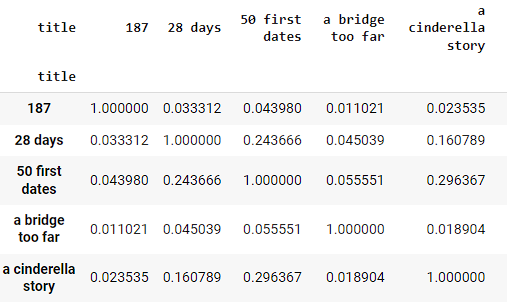
\includegraphics[height=5.5cm]{figures/similarity(item).png}
        \caption{Similarity matrix}
        \label{similarity(item)}
\end{figure}

\item \textbf{\textit{STEP 4: Recommendation Function}}
This is the last step which is based on building the recommendation system. Before proceeding with the construction of the function, the similarity scores are standardized and normalized by multiplying the similarity score of the movies with the standardized ratings. The ratings are standardized by subtracting the mean of the ratings which is 2.5.

Further, the standardized ratings are sorted and arranged so that the most similar movies are recommended. Given below \ref{recommend(item)} are the recommendations of the movie \textit{Jaws} with the corresponding similarity scores
\begin{figure}[h]
        
        \centering
        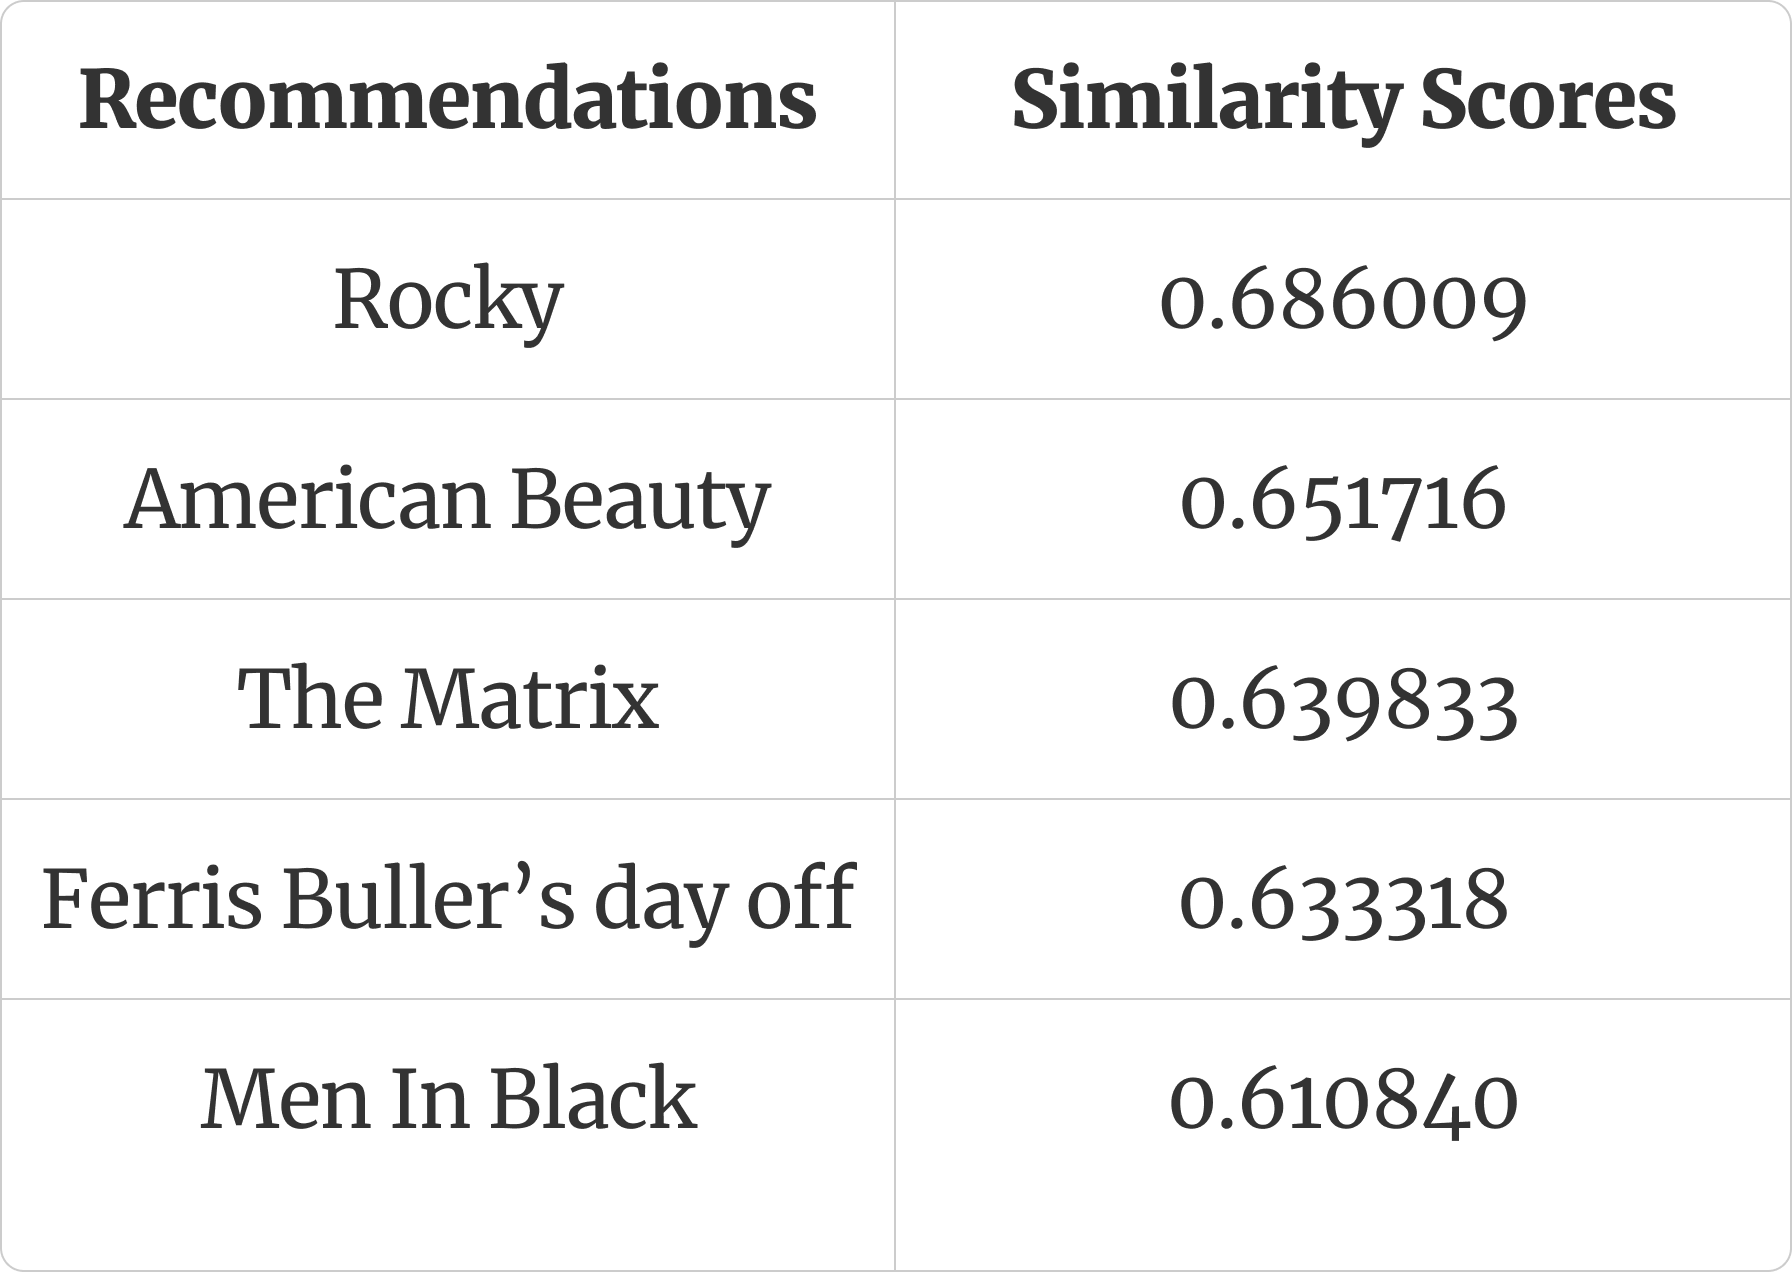
\includegraphics[height=3.4cm]{figures/recommend(item).png}
        \caption{Recommendations of the movie with similarity score}
        \label{recommend(item)}
\end{figure}

The function is so built that if any movies are not a part of the dataset then the most rated movies are recommended instead

\begin{figure}[H]
        
        \centering
        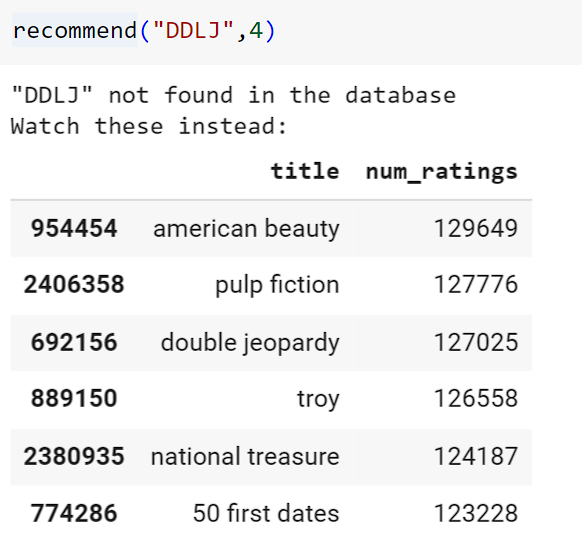
\includegraphics[height=4.5cm]{figures/not_in_db.png}
        \caption{Movie not found in the database}
        \label{not in db}
\end{figure}
\end{itemize}


\subsection{Singular Value Decomposition:}
    \vspace{2pt}
    
    \begin{itemize}
        \item \textbf{\textit{STEP 1: User Matrix and Singular Value Decomposition}}: This step focuses on building the user-movie correlation matrix based on the ratings given by users to all the movies. 
     This step particularly decomposes or breaks down the user-movie matrix into three matrices, namely, \( U \), \( \Sigma \), and \( V^T \). The "U" matrix represents how users are related to latent features. The latent features are the features that make up the movie, i.e., it can be anything from genre to cast to characters. Any such feature that adds value to a movie is called a latent feature.

\begin{figure}[H]
        
        \centering
        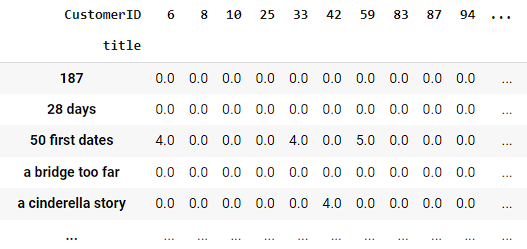
\includegraphics[height=4cm]{figures/user_movie.png}
        \caption{User-Movie Matrix}
        \label{User_movie}
\end{figure}

So the  \( U \) matrix represents the extent of association of each user with the features of a movie. The rows contain users and the columns contain the features of the movies. The values of this matrix are called \textit{left singular values}

\begin{figure} [H]
    \centering
    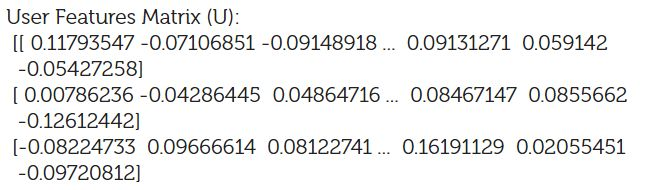
\includegraphics[height=2.5cm]{User_matrix.jpg}
    \caption{User Feature Matrix}
    \label{user}
\end{figure}

The \( V \) matrix represents the association between the movies and the features. The rows have movies and the columns consist of the features. 

\begin{figure}[H]
    \centering
    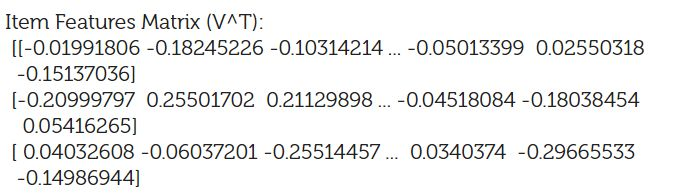
\includegraphics[height=2.5cm]{item_feature.jpg}
    \caption{Item Feature Matrix}
    \label{item}
\end{figure}

The \( \Sigma \) matrix is a diagonal matrix and contains values that depict the importance of the features. These values are arranged in descending order in the diagonal matrix. 
This process is called \textit{\textbf{Singular Value Decomposition.}}

\begin{figure}[H]
    \centering
    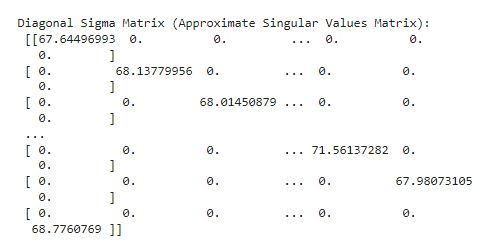
\includegraphics[height= 3.5cm]{sigma.jpg}
    \caption{\(Sigma\) Matrix}
    \label{fig:enter-label}
\end{figure}

\item \textbf{\textit{STEP 2: Reconstructed Matrix}}:
\vspace{2pt}
    This step crucially aims to find the dot product of the three decomposed matrices to find one matrix that is called the reconstructed matrix.

    The reconstructed matrix has movies in rows and user ratings in columns. The matrix is formed by predicting the ratings for the movies that the user has not seen by reading the patterns of all the watched movies. For the movies which the user has seen and rated the ratings in the matrix are the same as the original.

\item \textbf{\textit{STEP 3: Recommendation Function}}:

    The threshold is kept at the Top 5 rated movies in the entire movie dataset which are similar to the input movie, the recommendations are then made based on the predictions made by the algorithm
    
    In case the movies do not exist in the dataset then, the top movies are suggested
\begin{figure} [H]
    \centering
    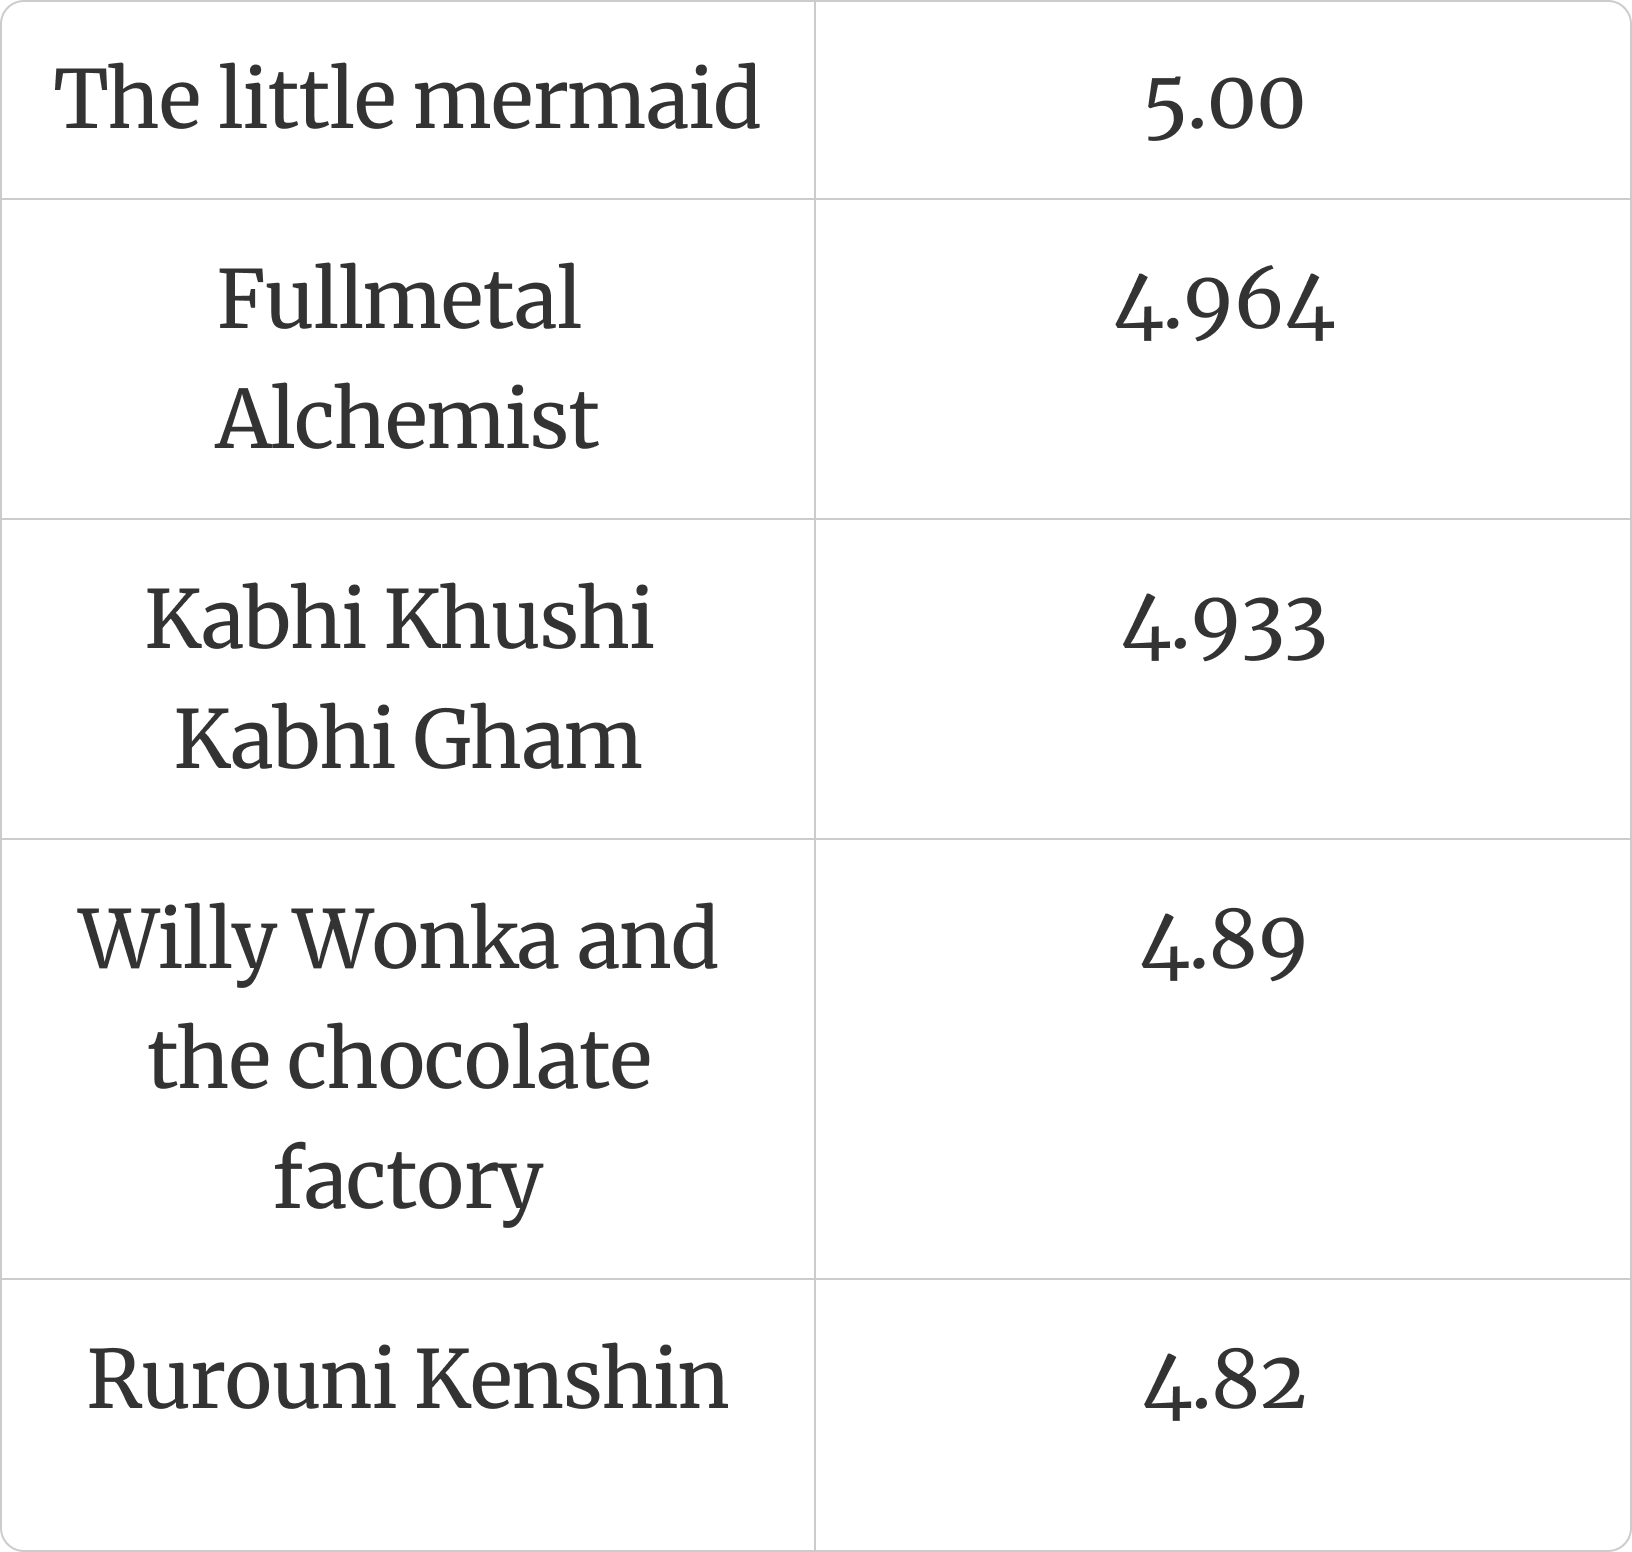
\includegraphics[width=4.5cm]{figures/svd_output.png}
    \caption{SVD output}
    \label{svd}
\end{figure}


\end{itemize}
\end{enumerate}


\subsection{Content-Based Filtering}
\begin{itemize}
    \item  \textbf{\textit{STEP 1: Create Tags}} 
    From the \textit{Netflix Titles} dataset, we will  create tags by combining the relevant columns. \textit{Description}, \textit{Listed in (genre)}, \textit{Cast}, \textit{Director} of each movie were merged in order to create the tags. The data frame \ref{tags} shows the created tags

\begin{figure}[H]
        
        \centering
        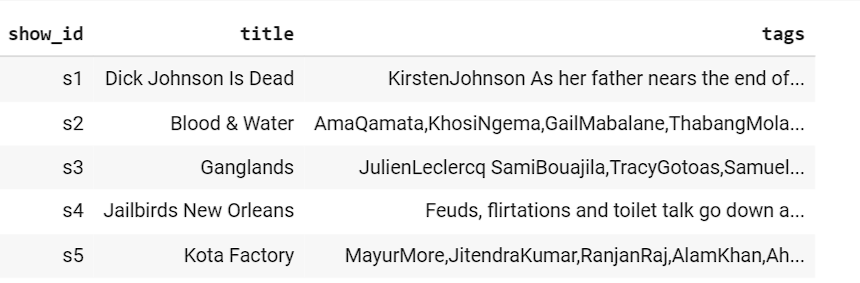
\includegraphics[height=3.2cm]{figures/tags.png}
        \caption{Dataframe containing tags of each movie}
        \label{tags}
\end{figure}


    \item  \textbf{\textit{STEP 2: Vectorization}}
    The next step is vectorization by the ‘Bag of words’ algorithm. This feature is used as an extraction technique that models text data for processing in information retrieval. This technique is applied to the previously created tags to numerical data for further processing.

    \item  \textbf{\textit{STEP 3: Similarity Scores}}
    The similarity score is calculated between the items to find the likeness in item characteristics. The items in a movie recommendation system are the movies and hence the similarity score is calculated to find out the extent of similarity between all the movies based on features like cast, description, title, director etc.

    \item  \textbf{\textit{STEP 4: Recommendation Function}}
    The last step aims at building the recommendation system based on the similarity score of the movies. The movie with the highest similarity score is recommended. The function is so built that if any movies are not a part of the dataset then the most rated movies are recommended instead.

\begin{figure}[H]
        
        \centering
        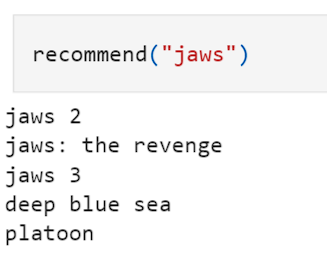
\includegraphics[height=3.7cm]{figures/recommend(content).png}
        \caption{Recommendations using Content-Based Filtering}
        \label{recommend(content)}
\end{figure}

\end{itemize}

\section{CONCLUSIONS}
Following figure \ref{conclude} shows the recommendations from all the three recommendation systems for the movie \textit{“Jaws”}

\begin{figure}[H]
        
        \centering
        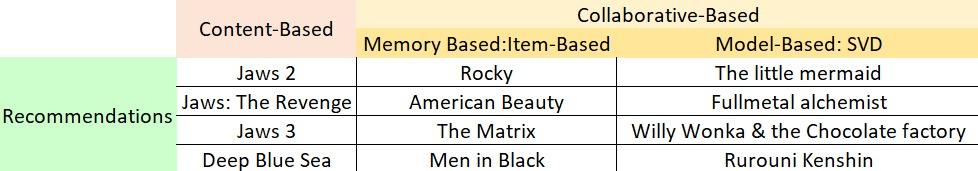
\includegraphics[height=2.5cm]{figures/conclude.jpg}
        \caption{Recommendations for Jaw using different techniques}
        \label{conclude}
\end{figure}

The recommendations made using content based recommendation system seem very similar whereas the recommendations made using SVD seem to be comparatively dissimilar

\section{LIMITATIONS}
\begin{itemize}
    \item Cold Start Problem- Incorporation of collaborative filtering does not solve the cold start problem. The algorithm will not be able to recommend movies to a new user.

    \item In the case of collaborative filtering, there was a huge amount of missing values in the data because many customers did not rate the movies. This leads to a problem of sparsity which reduces the accuracy of the model.

    \item It is difficult to apply user-based collaborative filtering due to the huge amount of customers.

    \item Due to the immense amount of data, computational efficiency was low. 

    \item In the case of content-based filtering, accuracy was comparatively low because of some discrepancies in the genre column and multiple missing values  
\end{itemize}


\section{FUTURE SCOPE}
\begin{itemize}
    \item The duration of user engagement with a movie  can be considered a vital feature instead of the ratings given by the user to make the model more robust

    \item Ensemble techniques and hybrid filtering can be used to get more accurate results

    \item More features like geography and demographics can be considered to improve the accuracy of the model

    \item Live data can be taken into account to continuously improve the model

\end{itemize}
\fontsize{8}{9}\selectfont


\bibliography{ResearchPaperBib}
\bibliographystyle{chicago}



\clearpage



\end{document}